This section covers the bag-of-tricks approach mentioned in Section~\ref{sec:design-fine-tuning-bagoftricks}, where multiple deep learning techniques covered throughout Chapters~\ref{ch:chapter-litsurvey} \& \ref{ch:chapter-design} are experimented with to determine which improve the performance of the model. Across each experiment, identical configurations are used to ensure that accurate comparisons can be made.

%%%%%%%%%%%%%%%%%%%%%%%%%%%%%%%%%%%%%%%%%%%%%

\section{Model Used}

The model described in Section~\ref{sec:design-cnn-model-decision} is used across all the experiments in this chapter, using both VGG19 and MobileNetV2 as the base model (except for the first experiment in Section~\ref{sec:evaluation-cnn-model-experiment}), a fully connected MLP with [512, 32, 2] neurons, a dropout layer using $p=0.2$, the Adam optimiser and whole images. Only the dataset, batch size, learning rate (0.001 or 0.0001), class weights, input size, weight initialisation and type of mammograms vary across the following experiments.

%%%%%%%%%%%%%%%%%%%%%%%%%%%%%%%%%%%%%%%%%%%%%

\section{Baseline}

Todo

%%%%%%%%%%%%%%%%%%%%%%%%%%%%%%%%%%%%%%%%%%%%%

\section{Base CNN Architectures}
\label{sec:evaluation-cnn-model-experiment}

Five different CNN model architectures (VGG19, ResNet50, InceptionV3, DenseNet121 and MobileNetV2) are tested out as the model's base (pre-trained on ImageNet) using the model described in Section~\ref{sec:design-cnn-model-decision}. For this test, the CBIS-DDSM dataset is used with whole images resized to 512 x 512 pixels, a batch size of 2 and a learning rate of 0.0001.\\

The results found in Table~\ref{tab:evaluation-cnn-models} clearly reveal that MobileNetV2 unlocks more performance than the other CNN architectures with a higher accuracy and F1 score. The original VGG19 architecture used during the the common pipeline development is outperformed by more efficient models like DenseNet121 or MobileNetV2 but outperforms the ResNet50 and InceptionV3. These results contradicts Falconi's results on the CBIS-DDSM dataset, who finds that ResNet50 outperforms MobileNetV2 \citep{Falconi2019}. However, MobileNetV2 still outperforms InceptionV3. These results may differ due to the different pre-processing techniques being used as Falconi uses cropped images around ROIs, whereas whole images are  used in  this experiment.\\

It is also worth noting  that using the model defined in Section~\ref{sec:design-cnn-model-decision} with the MobileNetV2 architecture already surpasses models that use traditional machine learning methods like SVMs with GLCM features, achieving 66.46\% accuracy against 63.03\% on the CBIS-DDSM dataset \citep{Sarosa2018}, confirming the points made in Section~\ref{sec:litsurvey-summary}. 

\begin{table}[h]
\centering
\begin{tabular}{@{}lcccc@{}}
\toprule
\textbf{CNN Architecture} &
  \multicolumn{1}{l}{\textbf{Overall Accuracy}} &
  \multicolumn{1}{l}{\textbf{Precision}} &
  \multicolumn{1}{l}{\textbf{Recall}} &
  \multicolumn{1}{l}{\textbf{F1 Score}} \\ \midrule
\textit{\textbf{VGG19}}       & 63.96\%          & 63.73\%          & 63.96\%          & 63.83\%          \\
\textit{\textbf{ResNet50}}    & 61.00\%          & 64.23\%          & 61.00\%          & 61.23\%          \\
\textit{\textbf{InceptionV3}} & 62.71\%          & 62.52\%          & 62.71\%          & 62.60\%          \\
\textit{\textbf{DenseNet121}} & 64.74\%          & 65.81\%          & 64.74\%          & 65.03\%          \\
\textit{\textbf{MobileNetV2}} & \textbf{66.46\%} & \textbf{66.25\%} & \textbf{66.46\%} & \textbf{66.33\%} \\ \bottomrule
\end{tabular}
\caption{Results achieved on the test set when using different CNN architectures as the base model pre-trained on ImageNet weights.}
\label{tab:evaluation-cnn-models}
\end{table}

However, observing the training and testing runtimes in Figure~\ref{fig:evaluation-CNN_models_experiment-runtimes} reveals that VGG19 takes the longest time to train with 3h50m, whereas the more efficient MobileNetV2 architecture takes 2h46. Additionally, prediction runtime is 2.3 times faster with MobileNetV2 compared to VGG19, which is more useful for clinics as mammogram diagnosis results can be returned faster.

\begin{figure}[h]
\centerline{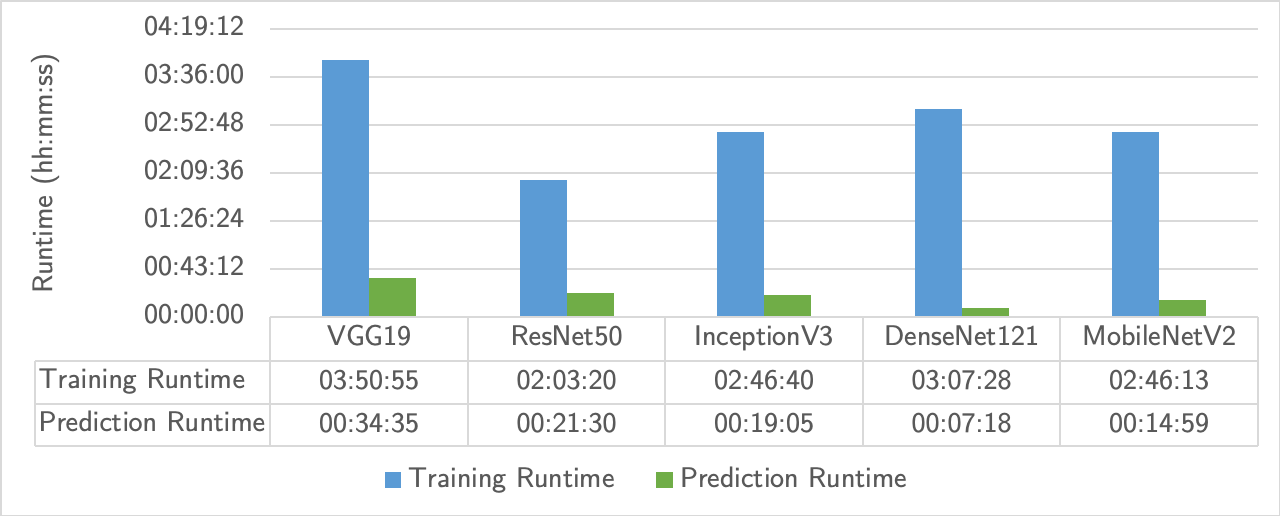
\includegraphics[width=\textwidth]{figures/evaluation/CNN_models_experiment/runtimes.png}}
\caption{\label{fig:evaluation-CNN_models_experiment-runtimes}Training and prediction runtimes when using different CNN architectures as the base model pre-trained on ImageNet.}
\end{figure}

%%%%%%%%%%%%%%%%%%%%%%%%%%%%%%%%%%%%%%%%%%%%%

\section{Class Weights}

Distinct variations of class weights are used on the CBIS-DDSM dataset to attempt to rectify the adverse effects that can be introduced by imbalanced datasets without going through the process of data augmentation, which would considerably slow down the training time by a factor equal to the number of new images generated.\\

Table~\ref{tab:evaluation-class-weights} reports the three class weight values that were tested using the imbalanced CBIS-DDSM dataset with whole images resized to 512 x 512 pixels, a batch size of 2 and a learning rate of 0.0001:
\begin{itemize}
    \item No class weights (dataset remains imbalanced);
    \item Balanced class weights:
    \begin{itemize}
        \item 0.907 for majority class (benign),
        \item 1.113 for minority class (malignant);
    \end{itemize}
    \item +50\% class weight for minority class:
    \begin{itemize}
        \item 1.0 for benign samples,
        \item 1.5 for malignant samples.
    \end{itemize}
\end{itemize}

\begin{table}[h]
\centering
\resizebox{\textwidth}{!}{%
\begin{tabular}{@{}llcccc@{}}
\toprule
\textbf{\begin{tabular}[c]{@{}l@{}}Base \\ model\end{tabular}} &
  \textbf{\begin{tabular}[c]{@{}l@{}}Class\\ weights\end{tabular}} &
  \multicolumn{1}{l}{\textbf{\begin{tabular}[c]{@{}l@{}}Overall \\ Accuracy\end{tabular}}} &
  \multicolumn{1}{l}{\textbf{Precision}} &
  \multicolumn{1}{l}{\textbf{Recall}} &
  \multicolumn{1}{l}{\textbf{F1 Score}} \\ \midrule
\multirow{3}{*}{\textit{\textbf{VGG19}}} &
  \textit{\textbf{None}} &
  62.25\% &
  63.66\% &
  62.25\% &
  62.58\% \\
 &
  \textit{\textbf{Balanced}} &
  63.96\% &
  63.94\% &
  63.96\% &
  63.95\% \\
 &
  \textit{\textbf{\begin{tabular}[c]{@{}l@{}}+50\%\\ minority\end{tabular}}} &
  61.15\% &
  62.16\% &
  61.15\% &
  61.45\% \\ \cmidrule(r){1-1}
\multirow{3}{*}{\textit{\textbf{MobileNetV2}}} &
  \textit{\textbf{None}} &
  65.83\% &
  66.33\% &
  65.83\% &
  66.01\% \\
 &
  \textit{\textbf{Balanced}} &
  \textbf{67.08\%} &
  \textbf{66.50\%} &
  \textbf{67.08\%} &
  \textbf{66.48\%} \\
 &
  \textit{\textbf{\begin{tabular}[c]{@{}l@{}}+50\%\\ minority\end{tabular}}} &
  65.05\% &
  65.19\% &
  65.05\% &
  65.12\% \\ \bottomrule
\end{tabular}%
}
\caption{Results achieved on the CBIS-DDSM test set when using different class weights (none, balanced and +50\% minority class) with VGG19 and MobileNet architectures as base model.}
\label{tab:evaluation-class-weights}
\end{table}

These results clearly depict how including balanced weights to the samples increases the accuracy across different base CNN models by 1.25-1.71\%, thus helping against the imbalanced dataset issue without resorting to techniques like data augmentation. However, a manual weight increase for the minority class decreases the accuracy by 0.78-1.1\%, revealing the complexity of finding the right parameters for balancing datasets as the 50\% weight increase for malignant samples made the dataset even more imbalanced. The normalised confusion matrices found in Figures~\ref{fig:evaluation-class_weights_experiment-none} and \ref{fig:evaluation-class_weights_experiment-balanced} expose how including class weights leads to the model being more confused as many malignant samples are classified as benign.

\begin{figure}[H]
\centerline{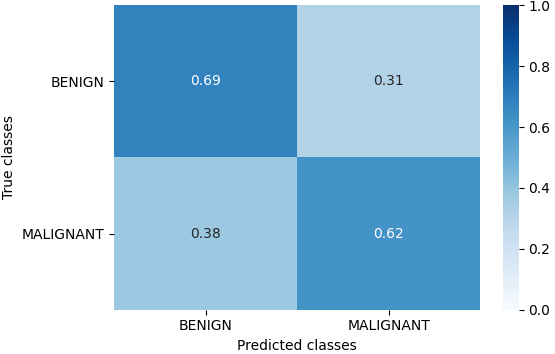
\includegraphics[width=0.75\textwidth]{figures/evaluation/class_weights_experiment/none.png}}
\caption{\label{fig:evaluation-class_weights_experiment-none}Normalised confusion matrix when no class weights are used with MobileNetV2 as the base model on the CBIS-DDSM dataset.}
\end{figure}

\begin{figure}[h]
\centerline{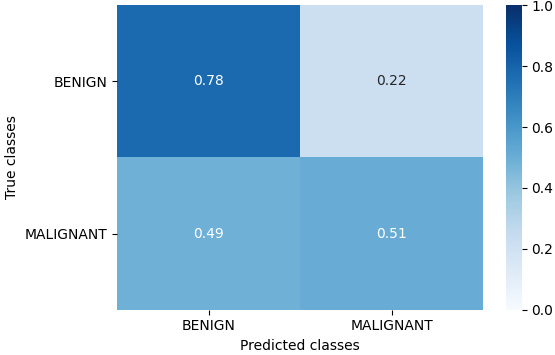
\includegraphics[width=0.75\textwidth]{figures/evaluation/class_weights_experiment/balanced.png}}
\caption{\label{fig:evaluation-class_weights_experiment-balanced}Normalised confusion matrix when balanced class weights are used with MobileNetV2 as the base model on the CBIS-DDSM dataset.}
\end{figure}

%%%%%%%%%%%%%%%%%%%%%%%%%%%%%%%%%%%%%%%%%%%%%

\section{Input Image Size}
\label{sec:evaluation-input-image-size}

Different image sizes are explored to determine their effect on the model's performance on the CBIS-DDSM dataset. For the smaller image sizes, larger batch sizes are used, whereas for the larger image sizes, smaller batch numbers are defined along with the extra convolutional and pooling layers mentioned in Section~\ref{sec:implementation-sequential-cnn-model} to make use of the larger image size as an attempt to learn lower-level features. The following image sizes are used:
\begin{itemize}
    \item 224 x 224 pixels (chosen as most CNNs pre-trained on ImageNet use this size) with a batch size of 8;
    \item 512 x 512 pixels with a batch size of 2;
    \item 1024 x 1024 pixels (with additional convolutional/pooling layers) with a batch size of 2.
\end{itemize}

\begin{table}[h]
\centering
\resizebox{\textwidth}{!}{%
\begin{tabular}{@{}llccccc@{}}
\toprule
\textbf{\begin{tabular}[c]{@{}l@{}}Base\\ Model\end{tabular}} &
  \textbf{\begin{tabular}[c]{@{}l@{}}Whole \\ Image \\ Size \\ (pixels)\end{tabular}} &
  \multicolumn{1}{l}{\textbf{\begin{tabular}[c]{@{}l@{}}Extra \\ conv/\\ pool \\ layers\end{tabular}}} &
  \multicolumn{1}{l}{\textbf{\begin{tabular}[c]{@{}l@{}}Overall\\ Accuracy\end{tabular}}} &
  \multicolumn{1}{l}{\textbf{Precision}} &
  \multicolumn{1}{l}{\textbf{Recall}} &
  \multicolumn{1}{l}{\textbf{F1 Score}} \\ \midrule
\multirow{3}{*}{\textbf{VGG19}}       & \textit{\textbf{224 x 224}}   & No  & 63.96\%          & 65.33\%          & 63.96\%          & 64.28\%          \\
                                      & \textit{\textbf{512 x 512}}   & No  & 64.59\%          & 64.44\%          & 64.59\%          & 64.51\%          \\
                                      & \textit{\textbf{1024 x 1024}} & Yes & 59.28\%          & \textbf{66.94\%} & 59.28\%          & 58.43\%          \\ \cmidrule(r){1-1}
\multirow{3}{*}{\textbf{MobileNetV2}} & \textit{\textbf{224 x 224}}   & No  & 62.56\%          & 62.38\%          & 62.56\%          & 62.46\%          \\
                                      & \textit{\textbf{512 x 512}}   & No  & \textbf{67.08\%} & 66.50\%          & \textbf{67.08\%} & \textbf{66.48\%} \\
                                      & \textit{\textbf{1024 x 1024}} & Yes & OOM              & OOM              & OOM              & OOM              \\ \bottomrule
\end{tabular}%
}
\caption{Results achieved on the test set when using different input image sizes on the CBIS-DDSM dataset.}
\label{tab:evaluation-image-size}
\end{table}

The results in Table~\ref{tab:evaluation-image-size} clearly expose the accuracy increase by using 512 pixels-wide input size rather than 224, with a 0.63\% increase on VGG19 and 4.52\% increase on MobileNetV2. However, further increasing the input size to 1024 pixels has no positive effect as the accuracy drops by 4.52\% on VGG19 and leads to an Out Of Memory (OOM) error on MobileNetV2, despite lowering the batch size to 1.\\

\begin{figure}[h]
\centerline{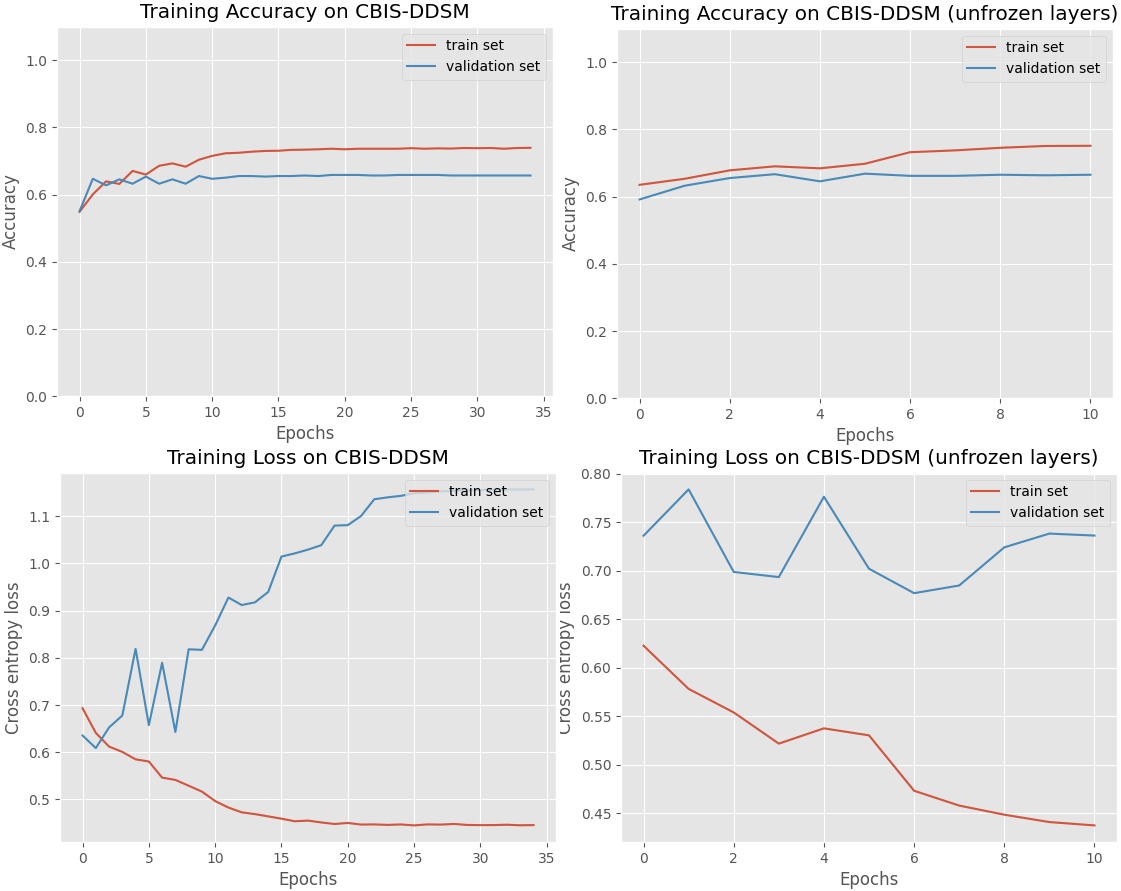
\includegraphics[width=1.2\textwidth]{figures/evaluation/image_size_experiment/training_summary.png}}
\caption{\label{fig:evaluation-image_size_experiment-training_summary}Evolution of the accuracy and loss during both training phases when testing 1024x1024 input size on VGG19.}
\end{figure}

Observing the evolution of the training accuracy and loss when using 1024 x 1024 pixels input size on VGG19 (see Figure~\ref{fig:evaluation-image_size_experiment-training_summary}), it can be seen that the validation loss increases while the training loss decreases and that both sets' training accuracies are increasing as well; which is a typical pattern of a model overfitting the data. Because the model is overfitting the data, a very high precision (66.94\%) but low recall (59.28\%) is witnessed in Table~\ref{tab:evaluation-image-size} for 1024x1024 input size, which is extremely detrimental as a BCD system that detects malignant cases as benign could lead to the death of the patient.\\

As expected, increasing the image size also increases the training runtime (see Figure~\ref{fig:evaluation-image_size_experiment-runtimes}), which is boosted by a factor of 2.4 when increasing from 224 to 512 pixels, and a factor of 2.8 from 512 to 1024 pixels on VGG19. However, another advantage of MobileNetV2 over VGG19 is that it scales better to larger input sizes as increasing the input from 224 to 512 pixels only raises the runtime by a factor of 1.54, and prediction times are quicker than VGG19 predictions (13.5 minutes on average for MobileNetV2 compared to 21.3 minutes for VGG19).

\begin{figure}[H]
\centerline{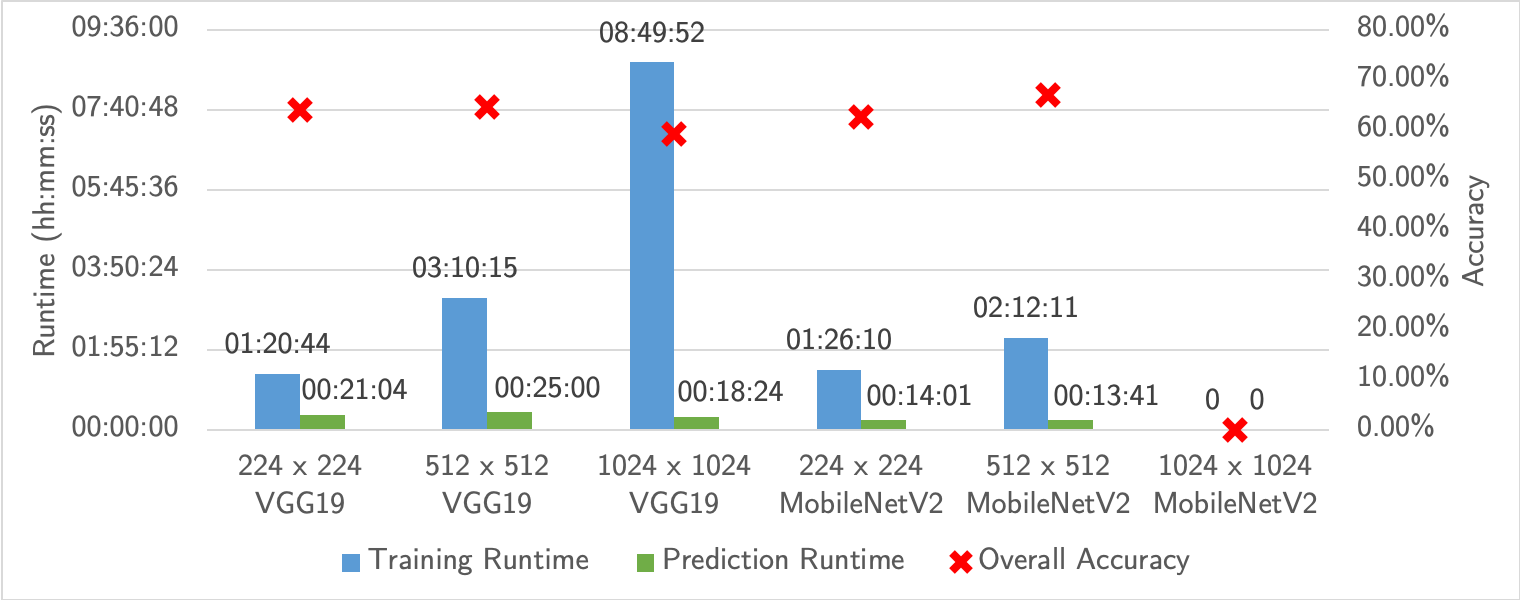
\includegraphics[width=\textwidth]{figures/evaluation/image_size_experiment/runtimes.png}}
\caption{\label{fig:evaluation-image_size_experiment-runtimes}Training and prediction runtimes when using different input image sizes.}
\end{figure}

Nevertheless, the accuracy/training runtime trade-off is not primordial in breast cancer detection as the primary goal is to develop a system that can correctly diagnose early forms of cancers in mammograms as accurately as possible, regardless of the runtime. Ultimately, prediction runtimes will matter when used in clinics.

%%%%%%%%%%%%%%%%%%%%%%%%%%%%%%%%%%%%%%%%%%%%%

\section{Varying Amounts of Transfer Learning}
\label{sec:evaluation-transfer-learning}

This experiment consists of expanding upon the concept of transfer learning. Instead of using a CNN pre-trained on ImageNet, weights of a model trained on a \textit{binarised} mini-MIAS dataset are transferred to the CBIS-DDSM dataset (see Section~\ref{sec:implementation-model-saving-minimiasbinary}). Four different experiments using an identical CNN architecture are tested to assess the effect of transfer learning from the binarised mini-MIAS dataset and ImageNet to the CBIS-DDSM dataset:
\begin{itemize}
    \item Transfer learning of all layer weights (MobileNetV2 and MLP layers instantiated with binary mini-MIAS weights);
    \item Transfer learning of fully connected layer weights (MLP layers instantiated with binary mini-MIAS weights, MobileNetV2 layers instantiated with ImageNet weights);
    \item Transfer learning of ImageNet weights only (MLP layers instantiated with random weights, MobileNetV2 layers instantiated with ImageNet weights);
    \item No transfer learning (MobileNetV2 and MLP connected layers instantiated with random weights).
\end{itemize}

\begin{table}[h]
\centering
\resizebox{\textwidth}{!}{%
\begin{tabular}{@{}lcccc@{}}
\toprule
\textbf{Transfer Learning} &
  \multicolumn{1}{l}{\textbf{Overall Accuracy}} &
  \multicolumn{1}{l}{\textbf{Precision}} &
  \multicolumn{1}{l}{\textbf{Recall}} &
  \multicolumn{1}{l}{\textbf{F1 Score}} \\ \midrule
\textit{\textbf{\begin{tabular}[c]{@{}l@{}}Full\\ mini-MIAS-binary\\ transfer learning\end{tabular}}}     & 63.18\% & 64.07\% & 63.18\% & 63.45\% \\ \cmidrule(r){1-1}
\textit{\textbf{\begin{tabular}[c]{@{}l@{}}MLP layers\\ mini-MIAS-binary \\ transfer learning\end{tabular}}} &
  \textbf{67.08\%} &
  \textbf{67.28\%} &
  \textbf{67.08\%} &
  \textbf{67.17\%} \\ \cmidrule(r){1-1}
\textit{\textbf{\begin{tabular}[c]{@{}l@{}}MobileNet layers\\ ImageNet\\ transfer learning\end{tabular}}} & 67.08\% & 66.50\% & 67.08\% & 66.48\% \\ \cmidrule(r){1-1}
\textit{\textbf{\begin{tabular}[c]{@{}l@{}}No transfer learning \\ (random weights)\end{tabular}}}        & 61.62\% & 61.00\% & 61.62\% & 61.17\% \\ \bottomrule
\end{tabular}%
}
\caption{Results achieved on the test set when using different amounts of transfer learning on the CBIS-DDSM dataset with the MobileNetV2 base model.}
\label{tab:evaluation-transfer-learning}
\end{table}

% \begin{table}[h]
% \centering
% \resizebox{\textwidth}{!}{%
% \begin{tabular}{@{}llcccc@{}}
% \toprule
% \textbf{\begin{tabular}[c]{@{}l@{}}Base\\ Model\end{tabular}} &
%   \textbf{\begin{tabular}[c]{@{}l@{}}Transfer\\ Learning\end{tabular}} &
%   \multicolumn{1}{l}{\textbf{\begin{tabular}[c]{@{}l@{}}Overall \\ Accuracy\end{tabular}}} &
%   \multicolumn{1}{l}{\textbf{Precision}} &
%   \multicolumn{1}{l}{\textbf{Recall}} &
%   \multicolumn{1}{l}{\textbf{F1 Score}} \\ \midrule
% \multirow{4}{*}{\textbf{VGG19 Common}} &
%   \textit{\textbf{\begin{tabular}[c]{@{}l@{}}Full \\ mini-MIAS-binary \\ transfer learning\end{tabular}}} &
%   57.87\% &
%   62.41\% &
%   57.88\% &
%   57.81\% \\ \cmidrule(lr){2-2}
%  &
%   \textit{\textbf{\begin{tabular}[c]{@{}l@{}}Fully \\ connected layers \\ mini-MIAS-binary \\ transfer learning\end{tabular}}} &
%   58.97\% &
%   60.43\% &
%   58.97\% &
%   59.33\% \\ \cmidrule(lr){2-2}
%  &
%   \textit{\textbf{\begin{tabular}[c]{@{}l@{}}ImageNet \\ transfer learning\end{tabular}}} &
%   59.44\% &
%   35.33\% &
%   59.44\% &
%   44.32\% \\ \cmidrule(lr){2-2}
%  &
%   \textit{\textbf{\begin{tabular}[c]{@{}l@{}}No transfer learning\\ (random weights)\end{tabular}}} &
%   60.37\% &
%   61.00\% &
%   60.37\% &
%   60.60\% \\ \cmidrule(r){1-2}
% \multirow{4}{*}{\textbf{MobileNetV2}} &
%   \textit{\textbf{\begin{tabular}[c]{@{}l@{}}Full \\ mini-MIAS-binary \\ transfer learning\end{tabular}}} &
%   63.18\% &
%   64.07\% &
%   63.18\% &
%   63.45\% \\ \cmidrule(lr){2-2}
%  &
%   \textit{\textbf{\begin{tabular}[c]{@{}l@{}}Fully \\ connected layers \\ mini-MIAS-binary \\ transfer learning\end{tabular}}} &
%   \textbf{67.08\%} &
%   \textbf{67.28\%} &
%   \textbf{67.08\%} &
%   \textbf{67.17\%} \\ \cmidrule(lr){2-2}
%  &
%   \textit{\textbf{\begin{tabular}[c]{@{}l@{}}ImageNet \\ transfer learning\end{tabular}}} &
%   \textbf{67.08\%} &
%   66.50\% &
%   \textbf{67.08\%} &
%   66.48\% \\ \cmidrule(lr){2-2}
%  &
%   \textit{\textbf{\begin{tabular}[c]{@{}l@{}}No transfer learning\\ (random weights)\end{tabular}}} &
%   61.62\% &
%   61.00\% &
%   61.62\% &
%   61.17\% \\ \cmidrule(r){1-2}
% \end{tabular}%
% }
% \caption{Results achieved on the test set when using different amounts of transfer learning on the CBIS-DDSM dataset using the custom MobileNetV2 and VGG19 models.}
% \label{tab:evaluation-transfer-learning}
% \end{table}

The results in Table~\ref{tab:evaluation-transfer-learning} clearly indicate that any form of transfer learning is better than random weight initialisation with such a small dataset. On the other hand, too much transfer learning by using all the weights from the model trained on the binary mini-MIAS dataset does not generalise well to the CBIS-DDSM dataset. The best performance came from initialising MobileNetV2 with ImageNet weights and the MLP layers with the MLP layer weights trained on the binary mini-MIAS, achieving an F1 score of 67.17\%. This was closely followed by again using ImageNet weights for MobileNetV2 and random weights for the MLP layers which reached the same overall accuracy but a lower F1 score (66.48\%).\\

The ImageNet weights transfer confirmed the performance that can be gained, as well the adaptive nature of CNNs when using knowledge learned from large general datasets for a more specific task like breast cancer detection.\\

\begin{figure}[h]
\centerline{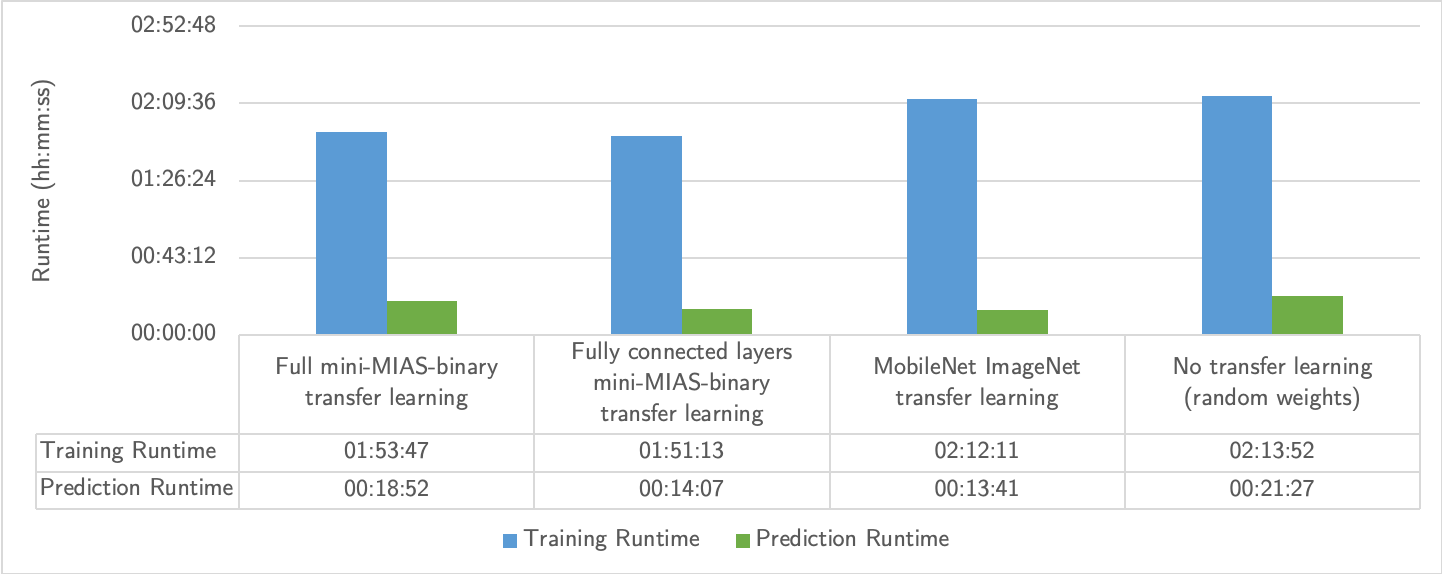
\includegraphics[width=\textwidth]{figures/evaluation/transfer_learning_experiment/runtimes.png}}
\caption{\label{fig:evaluation-transfer_learning_experiment-runtimes}Training and prediction runtimes when using different amounts of transfer learning with MobileNetV2 as a base model.}
\end{figure}

It is worth noting that training is slightly quicker when using weights from binary mini-MIAS (see Figure~\ref{fig:evaluation-transfer_learning_experiment-runtimes}) as the model converges more quickly towards a known solution. However, it is the early stopping conditions mentioned in Section~\ref{sec:design-validation-early-stopping} that dictate the training duration.

%%%%%%%%%%%%%%%%%%%%%%%%%%%%%%%%%%%%%%%%%%%%%

\section{Mammogram Types}

To assess how the model would adapt to samples from a single mammogram type only, the CBIS-DDSM dataset was separated into only masses samples and only calcifications samples (see Section~\ref{sec:ethics-datasets-cbisddsm} for samples). Three different experiments were tested:
\begin{itemize}
    \item All types of mammograms (masses + calcifications);
    \item Mass mammograms only;
    \item Calcification mammograms only.
\end{itemize}

\begin{table}[h]
\centering
\resizebox{\textwidth}{!}{%
\begin{tabular}{@{}llcccc@{}}
\toprule
\textbf{\begin{tabular}[c]{@{}l@{}}Base \\ Model\end{tabular}} &
  \textbf{\begin{tabular}[c]{@{}l@{}}Mammogram\\ type\end{tabular}} &
  \multicolumn{1}{l}{\textbf{\begin{tabular}[c]{@{}l@{}}Overall \\ Accuracy\end{tabular}}} &
  \multicolumn{1}{l}{\textbf{Precision}} &
  \multicolumn{1}{l}{\textbf{Recall}} &
  \multicolumn{1}{l}{\textbf{F1 Score}} \\ \midrule
\multirow{3}{*}{\textbf{VGG19}}       & \textit{\textbf{All}}            & 59.44\%          & 35.33\%          & 59.44\%          & 44.32\%          \\
                                      & \textit{\textbf{Masses}}         & 64.35\%          & 63.70\%          & 64.35\%          & 63.86\%          \\
                                      & \textit{\textbf{Calcifications}} & \textbf{66.67\%} & \textbf{67.05\%} & \textbf{66.67\%} & \textbf{66.80\%} \\ \midrule
\multirow{3}{*}{\textbf{MobileNetV2}} & \textit{\textbf{All}}            & \textbf{67.08\%} & \textbf{66.50\%} & \textbf{67.08\%} & \textbf{66.48\%} \\
                                      & \textit{\textbf{Masses}}         & 63.23\%          & 63.23\%          & 63.23\%          & 63.23\%          \\
                                      & \textit{\textbf{Calcifications}} & 63.12\%          & 64.57\%          & 63.12\%          & 63.39\%          \\ \bottomrule
\end{tabular}%
}
\caption{Results achieved on the test set when using different types of mammograms from the CBIS-DDSM dataset.}
\label{tab:evaluation-mammogram-types}
\end{table}

These results show that the model using VGG19 as a base model learns the data much better when masses and calcifications are separated, reaching 64.35\% and 66.67\% accuracy respectively on the test set, but only managing 59.44\% when using the full CBIS-DDSM dataset. Indeed, the normalised confusion matrix on the full CBIS-DDSM dataset indicates that all instances are classified as ``benign'', indicating that the model gets confused when dealing with multiple views and cannot tell benign and malignant cases from each other. This outcome is in line with Hepsag's results, which achieve higher accuracies when classifying either masses or calcifications on another dataset \citep{Hepsag2017}, and confirms Elter's claim that masses are harder to detect than calcifications \citep{Elter2009}.\\

However, the opposite effect is witnessed when MobileNetV2 is used as a base model, with an accuracy of 67.08\% reached when the full dataset is used and only 63.12\% and 63.23\% accuracy for calcifications and masses respectively, contradicting the previous results.

\begin{figure}[ht]
\centerline{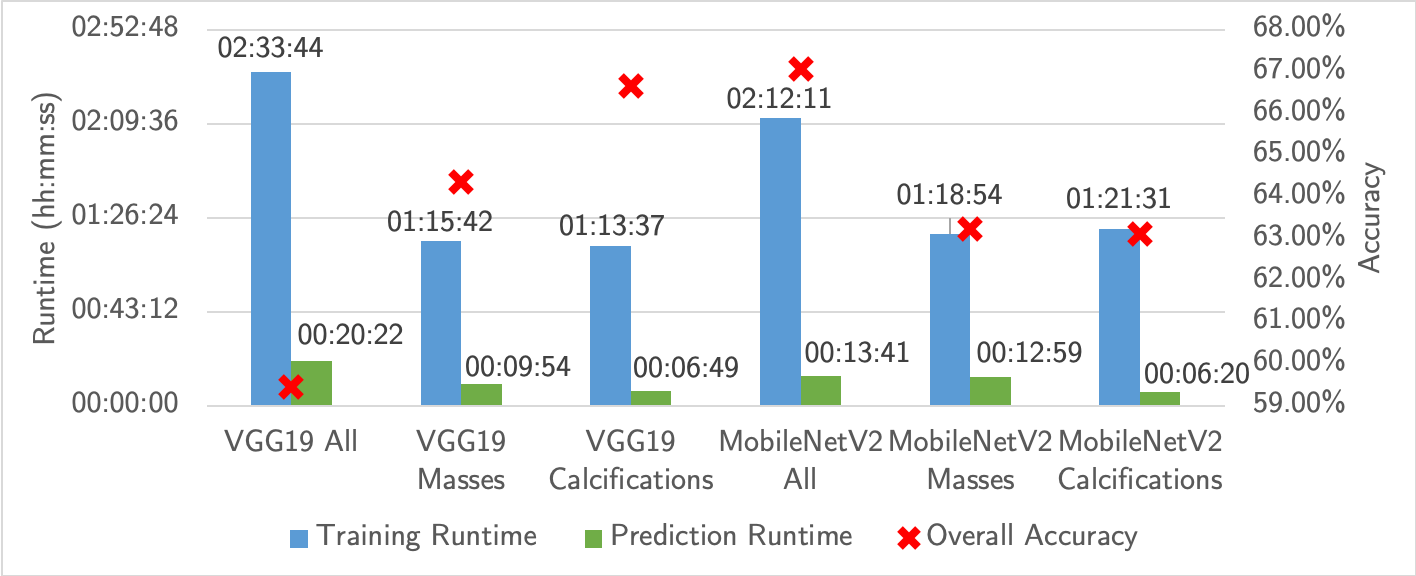
\includegraphics[width=\textwidth]{figures/evaluation/mammogram_type_experiment/runtimes.png}}
\caption{\label{fig:evaluation-mammogram_type_experiment-runtimes.png}Training and prediction runtimes when using different mammogram types.}
\end{figure}

In terms of runtime, training and prediction times are approximately twice as fast, since there is roughly twice less data after the dataset split (see Figure~\ref{fig:evaluation-mammogram_type_experiment-runtimes.png}).

%%%%%%%%%%%%%%%%%%%%%%%%%%%%%%%%%%%%%%%%%%%%%

\section{Results Summary}

Todo